\documentclass[a4paper,12pt]{report}

% Encodage et langue
\usepackage[utf8]{inputenc}
\usepackage[T1]{fontenc}
\usepackage[french]{babel}

% Mise en page
\usepackage{geometry}s
\geometry{margin=2.5cm}

% Packages utiles
\usepackage{graphicx}  % Pour les images
\graphicspath{{images/}}

\usepackage{amsmath, amssymb}  % Pour les maths
\usepackage[hidelinks]{hyperref}  % Pour les liens
\usepackage{float}  % Pour le placement des figures

\usepackage{enumitem} 

\title{ Introduction au Data Mining}
\author{DNJOMOU YONMBA WILFRIED LOIC CM-UDS-24SCI0999 \\
KENFACK LEONEL CM-UDS-17SCI0998\\
SAGUEU WAKAM DILANE CM-UDS-24SCI1040\\}
\date{Mars 2024}

\begin{document}

\maketitle

\renewcommand{\contentsname}{Table des matières}

\tableofcontents

\renewcommand{\chaptername}{Chapitre}

\chapter*{Introduction Générale}
Présentation générale du sujet et des objectifs du rapport.

\chapter{Définition et Enjeux du Data Mining}
Présentation du sujet et des objectifs du rapport.

    \section{Méthodologie}
    Description des méthodes utilisées.

\chapter{Approches et Processus du Data Mining}
    Le Data Mining est un processus complexe qui ne se limite pas à l’application d’algorithmes sur des données brutes. Il suit une démarche structurée qui permet d’extraire des connaissances exploitables à partir de vastes ensembles de données. Au fil des années, plusieurs méthodologies ont été développées pour encadrer cette démarche et garantir des résultats pertinents et reproductibles.\\
    Parmi les approches les plus influentes, on distingue le \textbf{processus KDD (Knowledge Discovery in Databases)}, qui pose les bases théoriques du Data Mining, et \textbf{CRISP-DM (Cross-Industry Standard Process for Data Mining)}, qui s’est imposé comme un standard industriel largement utilisé.\\
    Dans cette section, nous allons explorer ces deux méthodologies en détail. Nous verrons comment \textbf{KDD} structure l’extraction de connaissances d’un point de vue académique, et comment \textbf{CRISP-DM} adapte cette démarche aux besoins des entreprises en proposant un cadre plus opérationnel et itératif.

    \section{Le processus de découverte de connaissances (KDD)}
        Face à l'énorme quantité de données stockées dans des fichiers, des bases de données et autres référentiels, il est de plus en plus important, voire nécessaire, de développer des outils performants d'analyse et d'interprétation de ces données, ainsi que d'extraction de connaissances pertinentes susceptibles d'aider à la prise de décision.
        L'exploration de données, également appelée découverte de connaissances dans les bases de données (KDD: Knowledge Discovery in Databases), désigne l'extraction non triviale d'informations implicites, jusqu'alors inconnues et potentiellement utiles, à partir de données stockées dans des bases de données. Bien que le data mining et la découverte de connaissances dans les bases de données (KDD) soient souvent considérées comme des synonymes, le data mining fait en réalité partie du processus de découverte de connaissances. La figure suivante (Figure 2.1) illustre la fouille de données comme une étape d'un processus itératif de découverte de connaissances.\\
        \clearpage

        \begin{figure}[]
            \centering
            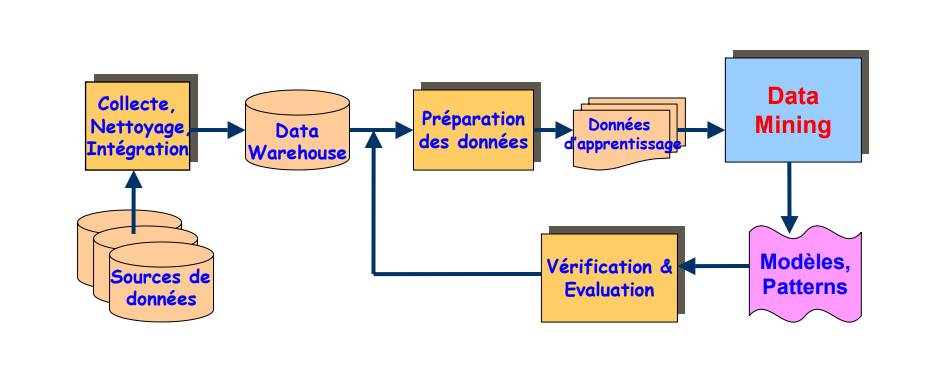
\includegraphics[width=0.75\textwidth]{KDD_data_mining}
            \caption{Data mining : coeur de KDD.}
            \label{fig:mesh1}
        \end{figure}        

        Le processus de découverte de connaissances dans les bases de données comprend plusieurs étapes, allant de la collecte de données brutes à la production de nouvelles connaissances. Ce processus itératif comprend les étapes suivantes.

        \begin{itemize}
            \item \textbf{Nettoyage des données} : il s’agit d’une phase au cours de laquelle les données parasites et les données non pertinentes sont supprimées de la collection.
            \item \textbf{Intégration des données} : à ce stade, plusieurs sources de données, souvent hétérogènes, peuvent être combinées en une source commune.
            \item \textbf{Sélection des données} : à cette étape, les données pertinentes pour l’analyse sont sélectionnées et extraites de la collecte de données.
            \item \textbf{Transformation des données} : également appelée consolidation des données, il s’agit d’une phase au cours de laquelle les données sélectionnées sont transformées sous des formes adaptées à la procédure d’exploration.
            \item \textbf{Exploration des données} : étape cruciale où des techniques astucieuses sont appliquées pour extraire des modèles potentiellement utiles.
            \item \textbf{Évaluation des modèles} : à cette étape, des modèles strictement intéressants représentant les connaissances sont identifiés sur la base de mesures données.
            \item \textbf{Représentation des connaissances} : phase finale au cours de laquelle les connaissances découvertes sont représentées visuellement à l’utilisateur. Cette étape essentielle utilise des techniques de visualisation pour aider les utilisateurs à comprendre et à interpréter les résultats de l’exploration des données. \\
        
        \end{itemize}

        Il est courant de combiner certaines de ces étapes. Par exemple, le nettoyage et l'intégration des données peuvent être réalisés conjointement lors d'une phase de prétraitement afin de générer un entrepôt de données. La sélection et la transformation des données peuvent également être combinées lorsque la consolidation des données résulte de la sélection ou, comme dans le cas des entrepôts de données, lorsque la sélection est effectuée sur des données transformées.

        Le KDD est un processus itératif. Une fois les connaissances découvertes présentées à l'utilisateur, les mesures d'évaluation peuvent être améliorées, l'exploration peut être affinée, de nouvelles données peuvent être sélectionnées ou transformées, ou de nouvelles sources de données peuvent être intégrées, afin d'obtenir des résultats différents et plus pertinents.

        Le data mining tire son nom des similitudes entre la recherche d'informations précieuses dans une grande base de données et l'extraction de minerais précieux. Ces deux techniques impliquent soit de passer au crible une grande quantité de matériaux, soit de sonder ingénieusement ces matériaux pour identifier précisément où se trouvent les valeurs. Il s'agit toutefois d'une appellation erronée, car l'extraction de l'or dans les roches est généralement appelée « extraction d'or » et non « extraction de roches ». Par analogie, l'exploration de données aurait donc dû être appelée « exploration de connaissances ». Néanmoins, l'exploration de données est devenue le terme courant et, très rapidement, une tendance qui a même éclipsé des termes plus généraux tels que la découverte de connaissances dans les bases de données (KDD), qui décrit un processus plus complet. D'autres termes similaires font référence à l'exploration de données : dragage de données, extraction de connaissances et découverte de modèles.

    \section{la méthodologie CRISP-DM}
        Développée par IBM dans les années 60, la méthodologie CRIPS-DM était conçue initialement pour des projets de Data Mining. Aujourd'hui elle est majoritairement utilisé dans les équipes de data science pour gérer les projets d’exploration et d’analyse des données.\\
        CRISP-DM, qui signifie Cross-Industry Standard Process for Data Mining, est une méthode mise à l'épreuve sur le terrain permettant d'orienter les travaux d'exploration de données.
        \begin{itemize}
            \item En tant que \textbf{méthodologie}, CRISP-DM comprend des descriptions des phases typiques d'un projet et des tâches comprises dans chaque phase, et une explication des relations entre ces tâches.
            \item En tant que \textbf{modèle de processus}, CRISP-DM offre un aperçu du cycle de vie de l'exploration de données.
        \end{itemize}
        
        \clearpage
        \begin{figure}[htbp]
                \centering
                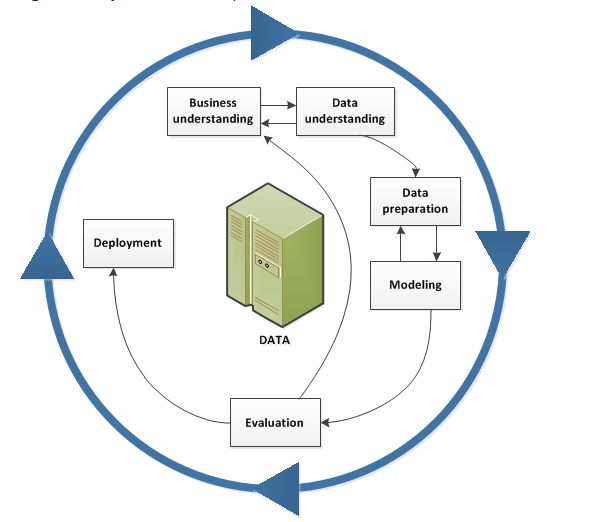
\includegraphics[width=0.75\textwidth]{crispdm}
                \caption{Le cycle de vie de l'exploration des données.}
                \label{fig:mesh1}
        \end{figure} 

        \subsection{Les étapes de CRISP-DM}
        Le modèle de cycle de vie comporte six(6) phases dotées de flèches indiquant les dépendances les plus importantes et les plus fréquentes entre les phases. La séquence des phases n'est pas strictement établie. De fait, les projets, pour la plupart, passent d'une phase à l'autre en fonction des besoins. 

            \subsubsection{Etape 1 : La compréhension du besoin client ou business understanding}
            Dans cette phase initiale, l’équipe de data science travaille en collaboration avec les parties prenantes afin de comprendre les objectifs commerciaux, les exigences, les contraintes du projet ainsi que les bénéfices attendus.\\ 
            Les ressources nécessaires pour réaliser le projet, tels que le budget, les compétences techniques et l'accès aux données, sont évalués. Les problèmes à résoudre sont identifiés et les critères permettant de mesurer le succès du projet sont définis. \\
            Cette étape est essentielle pour garantir la bonne atteinte des objectifs du projet.
    
            \subsubsection{Etape 2 : La compréhension des données ou data understanding}
            Cette phase consiste à collecter, explorer et évaluer toutes les données disponibles pour le projet. L'équipe de data science analyse ces dernières pour comprendre leur structure, leur qualité, leurs éventuels problèmes, leur pertinence et leur disponibilité. \\
            Cela permet d’identifier les valeurs manquantes, ou les erreurs qui pourraient affecter les analyses suivantes. Elle se concerte ensuite avec les experts métiers pour identifier des pistes de résolution des problèmes constatés et ainsi aider à interpréter les données.
    
            
            \subsubsection{Etape 3 : La préparation des données}
            Une fois que les données ont été évaluées, il faut à présent sélectionner les variables et les échantillons pertinents pour l’analyse, en fonction des objectifs qui ont été fixés.\\ 
            Les données sont ensuite nettoyées et, si nécessaire, transformées. Cela peut inclure la gestion des valeurs manquantes, l'échantillonnage des données et la création de variables dérivées. Si plusieurs sources de données sont utilisées, elles sont intégrées pour créer un ensemble de données cohérent.\\ 
            Cette étape monopolise plus de la moitié du temps sur l’ensemble du projet.
            
            \subsubsection{Etape 4 : La modélisation ou modeling}
            Dans cette phase, à partir de techniques d'analyse des données, l’équipe de data science construit des modèles prédictifs ou des modèles descriptifs, en fonction des objectifs du projet. Plusieurs itérations ont lieu entre les étapes de préparation et de modélisation pour affiner l’utilisation de certains algorithmes particuliers. \\
            L’étape du modeling génère souvent plusieurs modèles de Data Mining qui répondent tous à la même problématique.
    
            \subsubsection{Etape 5 : L’évaluation}
            Une fois que les modèles ont été construits, ils sont évalués pour déterminer leur qualité et leur précision. Cette étape du cycle permet de s’assurer que le modèle permet d’atteindre les objectifs du projet. \\
            Les performances des modèles sont mesurées à l'aide de métriques appropriées et comparées aux critères de succès définis dans la première phase du cycle. Si les résultats ne répondent pas aux attentes ou s'il y a des problèmes identifiés, les étapes précédentes peuvent être révisées et répétées pour améliorer les performances du modèle
    
    
            \subsubsection{Etape 6 : Le déploiement}
            Enfin, les résultats du projet sont présentés aux parties prenantes et sont intégrés si nécessaire dans les systèmes existants pour aider la prise de décision. Cette phase implique souvent la création de rapports, de visualisations ou d'autres formes de communication pour rendre les résultats compréhensibles et utilisables par ceux qui ne seraient pas spécialistes des données. \\
            A cette étape, le modèle est performant et répond correctement à la problématique.

        \subsection{Une approche agile }
        Il est important de noter que la méthodologie CRISP-DM est itérative, ce qui signifie que les différentes phases peuvent être révisées et répétées en fonction des résultats et des besoins du projet.\\
        A chaque étape d’une itération, l’équipe rédige un document qui récapitule ce qui a été fait ou ce qui a été trouvé. Ce document est mis à jour à chaque itération pour fournir ensuite un livrable complet au client.

        
\chapter{ Principales Techniques du Data Mining}
Présentation du sujet et des objectifs du rapport.

\section{Exploration et prétraitement des données }

    \section{Types d’apprentissage}
    
        Il existe trois grandes approches en apprentissage automatique : l'apprentissage supervisé, qui utilise des données étiquetées pour prédire des résultats, l'apprentissage non supervisé, qui travaille sur des données non étiquetées pour découvrir des structures, et l'apprentissage semi-supervisé, qui combine les deux pour exploiter des données partiellement étiquetées. Chaque approche présente des nuances et excelle dans des domaines spécifiques.
        
        \subsection{Apprentissage supervisé}
        
        L'apprentissage \textbf{supervisé} repose sur des ensembles de données étiquetées, c’est-à-dire que chaque donnée d’entrée est associée à une sortie connue (comme une catégorie ou une valeur), permettant à l’algorithme d’apprendre à prédire ces sorties pour de nouvelles données. Ces ensembles de données sont conçus pour former ou « superviser » les algorithmes afin qu'ils classent les données ou prédisent les résultats avec précision. En utilisant des entrées et des sorties étiquetées, le modèle peut mesurer sa précision et apprendre au fil du temps.
        
        \subsubsection*{Objectif}
        
        \begin{itemize}
            \item  À partir des données \(\{(x_i, y_i) \in \mathcal{X} \times \mathcal{Y}, i = 1, \ldots, N\}\), où \(x_i\) représente les caractéristiques d’un exemple (comme des symptômes) et \(y_i\) son étiquette (comme un diagnostic), estimer les dépendances entre \(\mathcal{X}\) et \(\mathcal{Y}\).
            \item  On parle d'apprentissage \textbf{supervisé} car les \(y_i\) permettent de guider le processus d’estimation.
        \end{itemize}
        
        \subsubsection*{Exemples}
        
        \begin{itemize}
            \item  Prédire le risque d’infarctus à partir de données sur l’alimentation et l’âge d’un patient. Ici, \(x_i\) correspond à \(d\) attributs concernant le régime d’un patient, et \(y_i\) à sa catégorie (risque ou pas de risque).
            \item  Détecter des fraudes bancaires en analysant des transactions étiquetées comme frauduleuses ou non.
            \item  Applications : diagnostic médical, reconnaissance de caractères, prévision de la demande, etc.
        \end{itemize}
        
        \subsubsection*{Techniques}
        
        \begin{itemize}
            \item L'apprentissage supervisé peut être divisé en deux types de problèmes : la \textbf{classification} (ex. machines à vecteurs de support, arbres de décision, réseaux de neurones) et la \textbf{régression} (ex. régression linéaire, régression logistique).
        \end{itemize}
        
        \subsection{Apprentissage non supervisé}
        
        L'apprentissage \textbf{non supervisé} utilise des algorithmes pour analyser des données non étiquetées et identifier des modèles ou regroupements sans aucune indication préalable sur les résultats attendus. Ces algorithmes découvrent des structures cachées dans les données sans intervention humaine, d'où le terme « non supervisé ».
        
        \subsubsection*{Objectifs}
        
        \begin{itemize}
            \item  À partir des données \(\{x_i \in \mathcal{X}, i = 1, \ldots, N\}\), décrire l’organisation des données, extraire des sous-ensembles homogènes ou explorer des structures cachées.
        \end{itemize}
        
        \subsubsection*{Exemples}
        
        \begin{itemize}
            \item  Regrouper les clients d’un supermarché selon leurs habitudes d’achat. Ici, \(x_i\) représente un individu (adresse, âge, habitudes de courses, etc.).
            \item  Détecter des anomalies dans des données industrielles, comme des défauts de fabrication.
            \item  Applications : segmentation de marchés, catégorisation de documents, compression d’images, etc.
        \end{itemize}
        
        \subsubsection*{Techniques}
        
        \begin{itemize}
            \item Les techniques incluent le \textbf{clustering} (ex. k-means, clustering hiérarchique), l’\textbf{association} (ex. Apriori pour les règles d’association) et la \textbf{réduction de dimensionnalité} (ex. analyse en composantes principales - PCA).
        \end{itemize}
        
        \subsection{Apprentissage semi-supervisé}
        
        L'apprentissage \textbf{semi-supervisé} vise à exploiter un petit ensemble de données étiquetées \(\{(x_1, y_1), \ldots, (x_n, y_n)\}\) et un grand ensemble de données non étiquetées \(\{x_{n+1}, \ldots, x_N\}\), notamment lorsque l’étiquetage est coûteux ou chronophage. L’objectif est similaire à celui de l’apprentissage supervisé, mais en tirant parti des données non étiquetées pour améliorer la performance.
        
        \subsubsection*{Objectifs}
        
        \begin{itemize}
            \item  Utiliser les données étiquetées pour guider l’apprentissage tout en exploitant les données non étiquetées pour mieux comprendre la structure des données.
        \end{itemize}
        
        \subsubsection*{Exemples}
        
        \begin{itemize}
            \item  Classer des pages Web avec seulement quelques labels disponibles, le reste étant non étiqueté.
            \item  Améliorer la reconnaissance vocale en combinant quelques échantillons étiquetés à des données audio brutes.
            \item  Applications : traitement du langage naturel, vision par ordinateur, bioinformatique, etc.
        \end{itemize}
        
        \subsubsection*{Exemples de méthodes}
        
        \begin{itemize}
            \item Méthodes bayésiennes, machines à vecteurs de support (SVM) semi-supervisées, auto-encodeurs, etc.
        \end{itemize}
    
      \section{Tâches principales du Data Mining}
        Le data mining englobe plusieurs tâches clés visant à extraire des informations utiles et des motifs cachés à partir de grandes quantités de données. Ces tâches peuvent être réalisées à l'aide de différentes techniques d'apprentissage automatique, en fonction des objectifs et de la nature des données. Voici les principales tâches du data mining :
        
        \subsection{Classification}
        
        La \textbf{classification} est une des tâches importante du datamining. L’objectif est de construire un modèle qui permet de prédire si une instance de donnée est membre d’une classe prédéfinie.  Nous décrivons dans ce qui suit les notions de base partagées par la plupart des algorithmes utilisées dans la classification comme les arbres de décision, machines à vecteurs de support (SVM), réseaux de neurones, k-plus proches voisins (k-NN).

        \subsubsection{Principe général}


            \begin{itemize}
                \item  Objectif : apprendre un modèle à partir de données étiquetées pour prédire la classe d’objets inconnus.
                \item  Fonctionnement : le modèle est entraîné sur un ensemble de données où chaque exemple est associé à une classe, puis il est utilisé pour classer de nouvelles données.
            \end{itemize}
            {\\}
            La classification utilise un ensemble $D$ de données appelées ensemble d’apprentissage. Chaque donnée est typiquement représentée sous forme d’un vecteur d’attributs 
            $x = \langle x_1, x_2, \dots, x_m, y \rangle$ avec $y$ un attribut de classe. 
            
            L’objectif de la classification est d’entraîner un algorithme de classification $A$ sur l’ensemble $S$, pour trouver une bonne approximation d’une certaine fonction $f(x) = y$. La fonction approximative $Cl$ calculée est appelée classifieur. 
            
            L’évaluation de la précision de $Cl$ est faite sur un ensemble de données $T$ indépendant de $S$, appelé ensemble de test. Le classifieur sera par la suite capable de prédire la valeur de classe $y$ pour de nouvelles données $d$, en calculant $Cl(d)$ (Figure \ref{fig:classification}).
            
            \begin{figure}[h]
                \centering
                \includegraphics[width=0.9\textwidth]{schema_classification.png}
                \caption{Schéma général de la tâche de classification}
                \label{fig:classification}
            \end{figure}
        
        \subsubsection*{Exemples}

        \begin{itemize}
            \item  Détection de spam : classer les emails comme « spam » ou « non spam ».
            \item  Diagnostic médical : prédire si un patient a une maladie spécifique en fonction de ses symptômes.
            \item  Applications : reconnaissance d’images, analyse de sentiments, prévision de churn client.
        \end{itemize}

        \subsubsection{Évaluation de la performance de la classification}

        La performance de la classification est mesurée en fonction du nombre d'instances bien classées et mal classées par le modèle. Elle est évaluée généralement par la \textit{précision} et le \textit{taux d'erreur} :
        
        \begin{itemize}
            \item \textbf{Précision (Accuracy)} = $\frac{\text{Nombre d'instances bien classées}}{\text{Nombre total d'instances}}$
            \item \textbf{Taux d'erreur (Error rate)} = $\frac{\text{Nombre d'instances mal classées}}{\text{Nombre total d'instances}}$
        \end{itemize}
        
        Ces valeurs sont mesurées sur l'ensemble de test qui peut être construit par différentes méthodes :

         \begin{itemize}
            \item  {La méthode 2/3 Apprentissage, 1/3 Test} :  L'apprentissage est réalisé sur 2/3 de l'ensemble de données, tandis que le 1/3 est réservé pour le test.
            \item  {La méthode de validation croisée}   C'est une méthode qui consiste à diviser l'ensemble $D$ en $k$ parties disjointes $\{D_1, D_2, ... D_k\}$. Le processus suivant est répété $k$ fois (Figure 2.6) : construction d'un classificateur $Cl_i$ avec l'ensemble privé de $D_i$ ($D - D_i$), ensuite évaluation de la précision de $Cl_i$ en utilisant les données $D_i$. La précision globale est obtenue par la moyenne. Les ensembles construits de cette manière sont appelés \textit{cross validated committees}.
        \end{itemize}
  
        \subsubsection*{Techniques}

        \subsubsection*{a) Arbres de Décision}
        Les arbres de décision sont un algorithme d’apprentissage supervisé utilisé pour la classification et la régression, modélisant les décisions sous forme d’une structure arborescente. Ils sont particulièrement appréciés pour leur interprétabilité et leur polyvalence.\\

        Un arbre de décision est décision est un arbre où : 
        \begin{itemize}
            \item Noeud interne interne = un attribu
            \item Branche Branche d’un noeud = un test sur un attribut
            \item Feuilles Feuilles = classe donnée
        \end{itemize}

       Le processus repose sur une série de tests successifs sur les attributs des données. À chaque étape, un attribut est choisi pour partitionner les données, et cette division est répétée récursivement jusqu’à ce que les sous-ensembles soient suffisamment purs, c’est-à-dire qu’ils contiennent majoritairement des échantillons d’une seule classe.

Le critère central est la sélection de l’attribut qui maximise la pureté des sous-ensembles. Deux mesures courantes sont utilisées :
- Entropie : elle quantifie le désordre dans un ensemble. Une entropie faible indique une répartition homogène des classes.
- Indice de Gini : il mesure l’impureté. Un indice faible signifie que les classes sont bien séparées.

L’objectif est de minimiser ces métriques pour créer des partitions où les classes sont distinctes.

        \subsubsection*{b) Machines à Vecteurs de Support (SVM)}
        Les SVM cherchent à identifier un hyperplan qui sépare les données de deux classes avec la marge la plus large possible. Cet hyperplan est le plan qui maximise la distance aux points les plus proches de chaque classe, appelés vecteurs de support. La marge est la zone vide entre l’hyperplan et ces points.

Si les données ne sont pas linéairement séparables dans leur espace d’origine, les SVM utilisent des fonctions noyau (comme le noyau polynomial ou RBF) pour projeter les données dans un espace de dimension supérieure où une séparation linéaire devient possible.
        
        \subsubsection*{c) Réseaux de Neurones}
        Les réseaux de neurones sont des modèles d’apprentissage automatique inspirés du cerveau humain, composés de couches de neurones interconnectés pour traiter des données et apprendre des patterns complexes.
        Ils sont constitués de couches de neurones interconnectés : une couche d’entrée, une ou plusieurs couches cachées, et une couche de sortie. Chaque neurone calcule une combinaison linéaire de ses entrées (pondérées par des poids) et applique une fonction d’activation pour produire une sortie.

L’apprentissage consiste à ajuster les poids pour minimiser une fonction de perte, qui mesure l’écart entre les prédictions du réseau et les vraies étiquettes. Cet ajustement se fait via la rétropropagation du gradient, qui propage l’erreur de la sortie vers l’entrée pour mettre à jour les poids.
        
        \subsubsection*{d) k-Plus Proches Voisins (k-NN)}
        k-NN est un algorithme paresseux, c’est-à-dire qu’il ne construit pas de modèle explicite pendant l’entraînement. Pour classer une nouvelle donnée, il identifie les k échantillons les plus proches dans l’ensemble d’entraînement et attribue la classe majoritaire parmi ces voisins.

La proximité est généralement mesurée avec la distance euclidienne(\( \sqrt{\sum (x_i - y_i)^2} \)), mais d’autres métriques comme la distance de Manhattan peuvent être utilisées selon le contexte.

        \subsection{Clustering ( (Segmentation) )}
        
        Le \textbf{clustering} (ou regroupement) vise à regrouper des objets similaires en clusters, sans utiliser de classes prédéfinies. Il est utilisé pour découvrir des structures ou des motifs cachés dans des données non étiquetées.
        
        \subsubsection*{Principe général}
        
        \begin{itemize}
            \item  Objectif : identifier des groupes naturels dans les données, où les objets d’un même cluster sont plus similaires entre eux que ceux des autres clusters.
            \item  Fonctionnement : les algorithmes de clustering analysent les similitudes entre les objets et les regroupent en conséquence.
        \end{itemize}
        {\\}
        Formellement : Soit X un ensemble de N données décrites chacune par leurs P
        attributs, la segmentation consiste a créer une décomposition de cet ensemble
        en groupes telle que les données appartenant au même groupe se ressemblent,
        tandis que les données appartenant a deux groupes différents soient peu
        ressemblantes.{\\}{\\}
        Le problème de segmentation optimale en k groupes est NP-complet. Il faut
        donc chercher des algorithmes calculant une bonne décomposition, sans
        espérer être sûr de trouver la meilleure. On distingue essentiellement deux 
        types de méthodes «non hiérarchiques» ou «hiérarchques».
        L’outils de base dans cette tâche est la mesure de similarité entre les données.
        
        \subsubsection*{Mesures de similarité}

        La méthode de calcul de distance entre deux objets dépend essentiellement de
        la nature des données à segmenter (Euclidienne, Jaccard, Hamming,
        Menhatten, ...). La figure (Figure \ref{fig:distance_eulidienne}) présente un exemple de calcul de la distance
        euclidienne entre deux objets.
            
        \begin{figure}[h]
            \centering
            \includegraphics[width=0.9\textwidth]{schema_distance_eulidienne.png}
            \caption{Exemple de calcul de la distance euclidienne}
            \label{fig:distance_eulidienne}
        \end{figure}

        \subsubsection*{Approche non hiérarchique}

        L'ensemble d'objets est décomposé en groupes. L’algorithme le plus répandu
        dans cette approche est «k-means» . La méthode du choix de la
        valeur de k (nombre de centroides initial) est un champs d’investigation. Par
        défaut, k est choisi aléatoirement. Le critère d’arrêt peut être soit la stabilisation
        des objets, ou bien d’autre mesures comme l’inertie. 

\\
        \begin{enumerate}[leftmargin=*]
            \item Déterminer le nombre de Clusters \( K\)
            \item Prendre \( K \) objets arbitraires «~centroides~»
            \item Calculer les distances entre les objets et les centroides
            \item Grouper les objets selon la distance minimale
            \item Si aucun objet ne change de groupes, alors fin
            \item Sinon calculer les nouveaux centroides, aller à 4
        \end{enumerate}
        
        Principe général de l’algorithme \( k \)-means

        \subsubsection*{Approche hiérarchique}
        On décompose l'ensemble d'objets en une arborescence de groupes
        (dendogramme). Le principe consiste à débuter de N groupes, que l'on réduit à
        N-1, puis a N-2.... etc. On passe donc de k+1 a k groupes en regroupant deux
        groupes. 
        \\
        \begin{enumerate}[leftmargin=*]
            \item Calculer la matrice des distances
            \item Chaque objet représente un Cluster
            \item Regrouper les deux clusters les plus proches
            \item Mettre à jour la matrice des distances
            \item Si le nombre de Clusters = 1, fin Sinon, aller à 3
          \end{enumerate}
        
        Principe de base du clustering hiérarchique
        
        \subsubsection*{Exemples}

        
        \begin{itemize}
            \item  Segmentation de marché : regrouper les clients en fonction de leurs comportements d’achat.
            \item  Analyse de données sociales : identifier des communautés dans les réseaux sociaux.
            \item  Applications : compression d’images, recommandation de contenu, biologie (classification de gènes).
        \end{itemize}
        
        % \subsubsection*{Techniques}
        
        % \begin{itemize}
        %     \item K-means, DBSCAN, clustering hiérarchique, Gaussian Mixture Models (GMM).
        % \end{itemize}
      
      \subsection{Régression}

La \textbf{régression} est une tâche du data mining qui vise à prédire une valeur numérique continue en fonction d'une ou plusieurs variables prédictives. Contrairement à la classification, qui prédit des étiquettes de classe catégoriques, la régression modélise des fonctions à valeurs continues. Elle est particulièrement utile lorsque les variables prédictives sont également continues.

\subsubsection*{Principe général}

\begin{itemize}
    \item  Objectif : apprendre un modèle à partir de données étiquetées pour prédire une valeur numérique pour de nouvelles données.
    \item  Fonctionnement : le modèle est entraîné sur un ensemble de données où chaque exemple est associé à une valeur cible continue, puis il est utilisé pour prédire cette valeur pour de nouvelles instances.
\end{itemize}

La régression cherche à modéliser la relation entre une variable dépendante \( y \) (la variable à prédire) et une ou plusieurs variables indépendantes \( x_1, x_2, \dots, x_n \) (les prédicteurs). Le modèle de régression le plus simple est la régression linéaire, où la relation est supposée linéaire.

\subsubsection*{Techniques}

Les techniques de régression incluent :

\begin{itemize}
    \item \textbf{Régression linéaire} : modélise la relation entre les variables par une ligne droite. Pour un seul prédicteur, elle prend la forme \( y = w_0 + w_1 x \), où \( w_0 \) et \( w_1 \) sont les coefficients à estimer. Ces coefficients sont souvent estimés par la méthode des moindres carrés, qui minimise la somme des carrés des erreurs entre les valeurs observées et prédites. Les formules sont :
    \[
    w_1 = \frac{\sum_{i=1}^D (x_i - \bar{x})(y_i - \bar{y})}{\sum_{i=1}^D (x_i - \bar{x})^2}, \quad w_0 = \bar{y} - w_1 \bar{x}
    \]
    où \( \bar{x} \) et \( \bar{y} \) sont les moyennes des \( x_i \) et \( y_i \), respectivement.


    Exemple : Prédiction du salaire : estimer le salaire d’un employé en fonction de son expérience professionnelle.

    \begin{figure}[h!]
        \begin{minipage}[b]{0.5\textwidth}
            \centering
            \includegraphics[width=\textwidth]{images/linear_data.png} 
            \caption{Table Data}
        \end{minipage}%
        \begin{minipage}[b]{0.5\textwidth}
            \centering
            \includegraphics[width=\textwidth]{images/linear_representation.png} 
            \caption{2-D data on a scatter plot.}
        \end{minipage}
    \end{figure}

        % Début de la mise en page en deux colonnes
        \begin{minipage}[t]{0.48\textwidth} % Colonne de gauche (texte)
        \vspace{0pt} % Alignement vertical
        
        À partir des données ci-dessus, nous calculons :
        \[
        \bar{x} = 9{,}1 \quad \text{et} \quad \bar{y} = 55{,}4
        \]
        
        Nous obtenons :
        \[
        w_1 = \frac{(3 - 9{,}1)(30 - 55{,}4) + \cdots + (16 - 9{,}1)(83 - 55{,}4)}{(3 - 9{,}1)^2 + \cdots + (16 - 9{,}1)^2} = 3{,}5
        \]
        
        \[
        w_0 = 55{,}4 - (3{,}5)(9{,}1) = 23{,}6
        \]
        
        L'équation de la droite des moindres carrés :
        \[
        y = 23{,}6 + 3{,}5x
        \]
        
        \end{minipage}
        
    
       \begin{figure}[h]
            \centering
            \includegraphics[width=0.9\textwidth]{images/linear_regression.png}
            \caption{Exemple de régression linéaire}
            \label{fig:reg}
        \end{figure}

    \item \textbf{Régression linéaire multiple} :  La régression linéaire multiple implique l'utilisation de plusieurs variables prédictives.   Les données d'apprentissage sont de la forme :
    \[
    (\mathbf{X}_1, y_1),\ (\mathbf{X}_2, y_2),\ \dots,\ (\mathbf{X}_p, y_p)
    \]
    où :
    \begin{itemize}
        \item $\mathbf{X}_i \in \mathbb{R}^n$ : vecteur de données de dimension $n$
        \item $y_i$ : étiquette de classe associée
    \end{itemize}
    
    c'extension de la régression linéaire à plusieurs prédicteurs, de la forme \( y = w_0 + w_1 x_1 + w_2 x_2 + \dots + w_n x_n \). Elle permet de modéliser des relations plus complexes en tenant compte de plusieurs variables.

    \item \textbf{Régression non linéaire} : utilisée lorsque la relation entre les variables n’est pas linéaire. Par exemple, la régression polynomiale : \( y = w_0 + w_1 x + w_2 x^2 + w_3 x^3 \). Elle peut capturer des relations plus complexes mais nécessite plus de données et peut être sujette au surajustement.
  
    \item \textbf{Modèles linéaires généralisés} : incluent la régression logistique, qui modélise la probabilité d’un événement, et la régression de Poisson, pour des données de comptage. Ils étendent la régression linéaire à des distributions non normales.

    \item \textbf{Arbres de régression et arbres de modèle} : des arbres de décision où les feuilles prédisent des valeurs numériques. Les arbres de régression prédisent la moyenne des instances atteignant la feuille, tandis que les arbres de modèle utilisent des modèles de régression dans les feuilles. Ils sont utiles pour des données non linéaires et peuvent être plus précis que les modèles linéaires simples.
\end{itemize}

\subsubsection*{Évaluation de la performance}

La performance des modèles de régression est évaluée à l’aide de métriques telles que :

\begin{itemize}
    \item \textbf{Erreur quadratique moyenne (MSE)} : \(\frac{1}{n} \sum_{i=1}^n (y_i - \hat{y}_i)^2\)
    \item \textbf{Erreur absolue moyenne (MAE)} : \(\frac{1}{n} \sum_{i=1}^n |y_i - \hat{y}_i|\)
    \item \textbf{Coefficient de détermination (R²)} : \(1 - \frac{\sum_{i=1}^n (y_i - \hat{y}_i)^2}{\sum_{i=1}^n (y_i - \bar{y})^2}\)
\end{itemize}

Ces métriques sont calculées sur un ensemble de test indépendant pour évaluer la capacité du modèle à généraliser à de nouvelles données.

Il est également important de sélectionner les attributs pertinents pour éviter le surajustement et d’identifier les valeurs aberrantes qui peuvent fausser les résultats de la régression.

En conclusion, la régression est une technique puissante pour la prédiction numérique, offrant une gamme de modèles adaptés à différents types de données et de relations entre variables.  
        \subsection{Détection d’anomalies}

        \subsection{Extraction de règles d’association}
        
        L'\textbf{extraction de règles d’association} est une tâche fondamentale en fouille de données (data mining), visant à identifier des relations implicites et significatives entre les attributs dans de grandes bases de données. Introduite par Agrawal et al. , cette technique est particulièrement reconnue pour son application dans l’analyse du panier de marché. Elle permet, par exemple, de dégager des règles telles que « 70\% des clients achetant du lait et du thé achètent aussi du pain », utiles pour optimiser l’agencement des rayons, planifier des promotions ou gérer les stocks dans un objectif d’amélioration des profits.
        
        Dans ce contexte, une base de données transactionnelle est un ensemble de transactions, où chaque transaction représente un sous-ensemble d’attributs (ou items) achetés par un client. Une règle d’association est une implication conditionnelle de la forme \( X \rightarrow Y \), où \( X \) et \( Y \) sont des ensembles d’attributs disjoints, exprimant que l’occurrence de \( X \) dans une transaction est souvent associée à celle de \( Y \). Le problème est complexe en raison du nombre exponentiel d’attributs possibles et du volume des bases transactionnelles, qui peuvent contenir des millions de transactions sur des milliers d’attributs.
        
        % Ce chapitre explore les processus d’extraction des règles d’association dans un contexte binaire. Il est structuré comme suit : la problématique est exposée dans la Section \ref{sec:prob_assoc}, les définitions et principes de base, incluant l’algorithme APRIORI, sont présentés dans la Section \ref{sec:def_principes}, les représentations condensées des motifs fréquents sont abordées dans la Section \ref{sec:rep_condensees}, et une conclusion est donnée dans la Section \ref{sec:concl_assoc}.
        
        \subsubsection{Problématique}
        \label{sec:prob_assoc}
        
        Le cadre classique de la fouille des règles d’association peut être décrit ainsi : soit \( A = \{x_1, x_2, \dots, x_m\} \) un ensemble de \( m \) attributs (ou items), et \( E = \{e_1, e_2, \dots, e_n\} \) un ensemble de \( n \) transactions, chaque transaction \( e_i \) étant un sous-ensemble de \( A \). Chaque transaction est associée à un identifiant unique (TID, Transaction IDentifier). Un motif est un sous-ensemble de \( A \), et une règle d’association est une implication \( X \rightarrow Y \) (où \( Y \neq \emptyset \)), indiquant que les attributs de \( X \) tendent à apparaître avec ceux de \( Y \).
        
        Les mesures clés pour évaluer une règle sont :
        \begin{itemize}
            \item Le \textbf{support} d’un motif \( X \), défini par \( \text{Supp}(X) = \frac{|\{e \in E \mid X \subseteq e\}|}{|E|} \), soit la proportion de transactions contenant \( X \).
            \item Le \textbf{support} d’une règle \( X \rightarrow Y \), égal à \( \text{Supp}(X \cup Y) \).
            \item La \textbf{confiance} d’une règle, définie par \( \text{Conf}(X \rightarrow Y) = \frac{\text{Supp}(X \cup Y)}{\text{Supp}(X)} \), soit la proportion de transactions contenant \( Y \) parmi celles contenant \( X \).
        \end{itemize}
        
        Le problème consiste à identifier toutes les règles valides, c’est-à-dire celles dont le support et la confiance dépassent des seuils minimaux prédéfinis, \( \text{minsupp} \) et \( \text{minconf} \). Ce problème est décomposé en deux étapes \cite{HGN00} :
        \begin{enumerate}
            \item Trouver tous les \textbf{motifs fréquents}, i.e., les motifs dont \( \text{Supp}(X) \geq \text{minsupp} \).
            \item Générer les règles d’association valides à partir de ces motifs fréquents.
        \end{enumerate}
        
        La première étape est la plus coûteuse, car l’espace de recherche des motifs fréquents est exponentiel. Dans les bases fortement corrélées ou avec un \( \text{minsupp} \) faible, le nombre de motifs peut devenir ingérable, nécessitant des optimisations comme les représentations condensées.
        
        \subsubsection{Définitions et principes de base}
        \label{sec:def_principes}
        
        Soit \( K = (E, A, R) \) un contexte de fouille de données, où \( R \) est une relation binaire entre les transactions \( E \) et les attributs \( A \). Les définitions fondamentales sont les suivantes :
        \begin{itemize}
            \item Un \textbf{motif} \( X \subseteq A \) est un ensemble d’attributs.
            \item Un motif est \textbf{fréquent} si \( \text{Supp}(X) \geq \text{minsupp} \).
            \item Une \textbf{règle d’association} \( X \rightarrow Y \) est valide si \( \text{Supp}(X \cup Y) \geq \text{minsupp} \) et \( \text{Conf}(X \rightarrow Y) \geq \text{minconf} \).
        \end{itemize}
        
        \paragraph{L’algorithme APRIORI}
        
        L’algorithme \textbf{APRIORI} \cite{AS94} est une méthode pionnière pour extraire les motifs fréquents. Il repose sur la propriété d’anti-monotonicité du support : si un motif \( X \) est fréquent, tous ses sous-ensembles le sont aussi ; inversement, si \( X \) n’est pas fréquent, aucun de ses sur-ensembles ne l’est. Formellement :
        \begin{itemize}
            \item Si \( X \subseteq Y \), alors \( \text{Supp}(X) \geq \text{Supp}(Y) \).
            \item Si \( X \) est fréquent, tout \( X_1 \subseteq X \) l’est aussi.
            \item Si \( X \) n’est pas fréquent, tout \( X_2 \supseteq X \) ne l’est pas.
        \end{itemize}
        
        L’algorithme procède itérativement :
        \begin{enumerate}
            \item Initialisation : trouver les 1-motifs fréquents (\( F_1 \)).
            \item Pour chaque niveau \( k \geq 2 \) :
                \begin{enumerate}
                    \item Générer les candidats \( C_k \) à partir des motifs fréquents \( F_{k-1} \) (via une jointure et un élagage basé sur l’anti-monotonicité).
                    \item Calculer le support des candidats en parcourant la base.
                    \item Retenir les motifs fréquents \( F_k = \{c \in C_k \mid \text{Supp}(c) \geq \text{minsupp}\} \).
                \end{enumerate}
            \item Arrêt : lorsque \( F_{k-1} = \emptyset \).
        \end{enumerate}
        
        Le pseudo-code est le suivant :
        \begin{verbatim}
        Entrée : K (base transactionnelle), minsupp
        Sortie : F (ensemble des motifs fréquents)
        1: F_1 ← {1-motifs fréquents}
        2: for (k ← 2; F_{k-1} ≠ ∅; k++)
        3:     C_k ← Apriori-Gen(F_{k-1})
        4:     for all e ∈ E
        5:         C_E ← {c ∈ C_k | c ⊆ e}
        6:         for all c ∈ C_E
        7:             Supp(c)++
        8:         end for
        9:     F_k ← {c ∈ C_k | Supp(c) ≥ minsupp}
        10: end for
        11: Retourner F ← ∪_k F_k
        \end{verbatim}
        
        \paragraph{Génération des règles}
        
        À partir des motifs fréquents \( F \), pour chaque motif \( I \in F \), on génère les règles \( X \rightarrow Y \) (où \( I = X \cup Y \), \( Y \neq \emptyset \)) en vérifiant \( \text{Conf}(X \rightarrow Y) \geq \text{minconf} \). Une optimisation \cite{AS94} exploite la propriété suivante : si \( I_1 \rightarrow I \setminus I_1 \) est valide, alors toute règle avec une prémisse \( I_2 \subset I_1 \) l’est aussi, réduisant ainsi le nombre de règles à tester.
        
        \subsubsection{Représentations condensées}
        \label{sec:rep_condensees}
        
        L’extraction exhaustive des motifs fréquents peut être prohibitive en termes de temps et de mémoire. Les \textbf{représentations condensées} sont des sous-ensembles compacts de motifs fréquents permettant de dériver l’ensemble complet des motifs et leurs supports. Voici quelques approches :
        
        \paragraph{Motifs fermés fréquents}
        
        Un motif \( X \) est \textbf{fermé} si aucun sur-ensemble n’a le même support (\( \phi(X) = X \), où \( \phi \) est un opérateur de fermeture). L’ensemble des motifs fermés fréquents \( FF = \{X \subseteq A \mid \phi(X) = X, \text{Supp}(X) \geq \text{minsupp}\} \) est une représentation condensée \cite{PBTL99a}. L’algorithme CLOSE génère ces motifs efficacement.
        
        \paragraph{Motifs libres}
        
        Un motif \( X \) est \textbf{\( \delta \)-libre} s’il n’existe pas de règle \( X_1 \rightarrow X_2 \) basée sur \( X = X_1 \cup X_2 \) avec peu d’exceptions (\( \text{Supp}(X_1) - \text{Supp}(X_1 \cup X_2) \leq \delta \)) \cite{BB00}. L’ensemble \( \text{FreqFree}(E, \sigma, \delta) \) des motifs \( \delta \)-libres fréquents, combiné à sa bordure négative, offre une représentation \( \epsilon \)-adéquate \cite{BBR03}.
        
        \paragraph{Motifs essentiels}
        
        Un motif \( X \) est \textbf{essentiel} si son support disjonctif \( \text{Supp}(\vee X) \) diffère de celui de ses sous-ensembles directs \cite{CCL05}. L’union des motifs essentiels fréquents et de la bordure positive \( \text{Bd}^+(F) \) forme une couverture parfaite des motifs fréquents.
        
        \paragraph{Motifs non dérivables}
        
        Un motif \( I \) est \textbf{non dérivable} si son support ne peut être exactement déduit des supports de ses sous-ensembles via des règles d’inclusion-exclusion \cite{CG06}. L’ensemble \( \text{NDIRep} \) des motifs non dérivables fréquents est une représentation condensée.
        
        % \subsubsection{Conclusion}
        % \label{sec:concl_assoc}
        
        % L’extraction des règles d’association est essentielle pour révéler des relations cachées dans les données. La recherche des motifs fréquents, bien que coûteuse, est optimisée par les représentations condensées (motifs fermés, libres, essentiels, non dérivables), qui réduisent le nombre de motifs à traiter tout en conservant l’information nécessaire. Cependant, le grand nombre de règles générées reste un défi, menant à des approches comme les bases de règles, sous-ensembles minimaux permettant de dériver toutes les règles valides, sujet exploré dans d’autres travaux.

        


\chapter{Outils et Langages utilisés}
Il existe une multitude d’outils pour effectuer des tâches de Data Mining. Voici quelques-uns des outils les plus populaires, chacun offrant ses propres fonctionnalités et avantages :

    \section{Python}
    \textbf{Python} est un \emph{langage de programmation} polyvalent largement utilisé dans le domaine de la Data Science et du Data Mining. Il offre une vaste gamme de bibliothèques et de frameworks tels que Pandas, NumPy, scikit-learn, TensorFlow, etc., qui permettent d’effectuer diverses tâches d’analyse de données, de modélisation et de visualisation.

    \section{RapidMiner}
    \textbf{RapidMiner} est une plateforme de Data Science qui propose une interface conviviale pour la préparation des données, la modélisation, l’évaluation et le déploiement des modèles. Il offre une grande variété d’algorithmes de Data Mining et de fonctionnalités de traitement des données, ce qui en fait un choix populaire parmi les professionnels du domaine.

    
    \section{WEKA}
    \textbf{WEKA} (Waikato Environment for Knowledge Analysis) est un logiciel open source développé par l'Université de Waikato. L'outil de data mining est basé sur Java et peut être utilisé avec Windows, MacOS et Linux. Reconnu pour ses capacités étendues d'apprentissage machine, il prend en charge toutes les principales tâches d'exploration de données telles que la mise en grappe, l'association, la régression ou la classification. L'interface utilisateur graphique facilite l'accès au logiciel. En outre, WEKA offre la connexion aux bases de données SQL et peut traiter les données demandées. La force de WEKA réside dans la classification : l'outil de data mining est connu pour ses nombreuses classifications, y compris les réseaux neuronaux artificiels, les arbres de décision, les algorithmes ID3 ou C4.5. Cependant, WEKA est moins puissant dans d'autres techniques telles que l'analyse cluster. Seules les procédures les plus importantes sont proposées ici. Un autre inconvénient : WEKA peut rencontrer des problèmes de traitement si de grandes quantités de données doivent être manipulées ; en effet, l'outil d'exploration de données essaye de les charger toutes dans la mémoire de travail. Pour s'en sortir, WEKA propose une ligne de commande simple qui facilite le traitement de grandes quantités de données. 

    
    \section{Orange}
    \textbf{Orange} est une suite logicielle open-source qui offre des outils de visualisation de données, de modélisation prédictive et de Data Mining. Il propose une interface graphique intuitive qui permet aux utilisateurs de créer et d’exécuter des workflows de traitement de données sans écrire de code, ce qui le rend accessible aux débutants et aux experts.

    
    \section{KNIME}
    \textbf{KNIME} est une plateforme open-source qui permet aux utilisateurs de créer des workflows visuels pour l’analyse des données et le déploiement de modèles. Il propose une large gamme de modules pour le Data Mining, la manipulation de données, la visualisation et plus encore. KNIME est apprécié pour sa flexibilité et sa capacité à intégrer des outils et des technologies externes.
    
    \section{SAS}
    \textbf{SAS Enterprise Miner} est une solution logicielle robuste conçue pour l’analyse prédictive et le Data Mining. Il offre une large gamme d’algorithmes de modélisation avancés, une interface conviviale pour la création de workflows et des fonctionnalités de déploiement de modèles. SAS Enterprise Miner est largement utilisé dans les entreprises pour résoudre des problèmes complexes liés à l’analyse de données.



\chapter{Défis et Limites du Data Mining}
Présentation du sujet et des objectifs du rapport.

\section{Méthodologie}
Description des méthodes utilisées.



\bibliographystyle{plain} % Style de la bibliographie
\bibliography{references} % Fichier BibTeX (references.bib)

\end{document}

